% This file is generated by the MATLAB m-file laprint.m. It can be included
% into LaTeX documents using the packages epsfig and psfrag. It is accompanied
% by a postscript file. A sample LaTeX file is:
%    \documentclass{article} \usepackage{epsfig,psfrag}
%    \begin{document}\begin{figure}% This file is generated by the MATLAB m-file laprint.m. It can be included
% into LaTeX documents using the packages epsfig and psfrag. It is accompanied
% by a postscript file. A sample LaTeX file is:
%    \documentclass{article} \usepackage{epsfig,psfrag}
%    \begin{document}\begin{figure}% This file is generated by the MATLAB m-file laprint.m. It can be included
% into LaTeX documents using the packages epsfig and psfrag. It is accompanied
% by a postscript file. A sample LaTeX file is:
%    \documentclass{article} \usepackage{epsfig,psfrag}
%    \begin{document}\begin{figure}% This file is generated by the MATLAB m-file laprint.m. It can be included
% into LaTeX documents using the packages epsfig and psfrag. It is accompanied
% by a postscript file. A sample LaTeX file is:
%    \documentclass{article} \usepackage{epsfig,psfrag}
%    \begin{document}\begin{figure}\input{subsidy}\end{figure}\end{document}
% See http://www.uni-kassel.de/~linne/ for recent versions of laprint.m.
%
% created by:           LaPrint version 2.03 (19.1.2000)
% created on:           13-Oct-2009 13:15:05
% options used:         / noextrapicture
% latex width:          12 cm
% factor:               0.8
% eps file name:        subsidy.eps
% eps bounding box:     15 cm x 11.25 cm
% comment:              
%
\begin{psfrags}%
\psfragscanon%
%
% text strings:
\psfrag{str03}[t][t]{x}%
\psfrag{str04}[b][b]{Subsidy factor: $-tanh(x-b)$}%
%
% xticklabels:
\psfrag{x01}[t][t]{-6}%
\psfrag{x02}[t][t]{-4}%
\psfrag{x03}[t][t]{-2}%
\psfrag{x04}[t][t]{0}%
\psfrag{x05}[t][t]{2}%
\psfrag{x06}[t][t]{4}%
\psfrag{x07}[t][t]{6}%
%
% yticklabels:
\psfrag{v01}[r][r]{-1}%
\psfrag{v02}[r][r]{-0.8}%
\psfrag{v03}[r][r]{-0.6}%
\psfrag{v04}[r][r]{-0.4}%
\psfrag{v05}[r][r]{-0.2}%
\psfrag{v06}[r][r]{0}%
\psfrag{v07}[r][r]{0.2}%
\psfrag{v08}[r][r]{0.4}%
\psfrag{v09}[r][r]{0.6}%
\psfrag{v10}[r][r]{0.8}%
\psfrag{v11}[r][r]{1}%
%
% Figure:
\resizebox{12cm}{!}{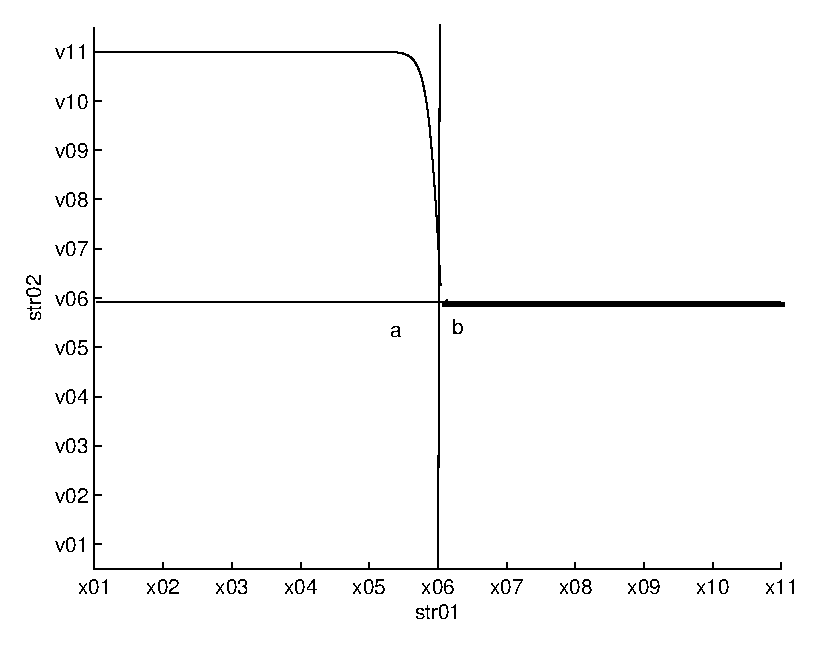
\epsfig{file=./stabilization/eps/subsidy.eps}}%
\end{psfrags}%
%
% End subsidy.tex
\end{figure}\end{document}
% See http://www.uni-kassel.de/~linne/ for recent versions of laprint.m.
%
% created by:           LaPrint version 2.03 (19.1.2000)
% created on:           13-Oct-2009 13:15:05
% options used:         / noextrapicture
% latex width:          12 cm
% factor:               0.8
% eps file name:        subsidy.eps
% eps bounding box:     15 cm x 11.25 cm
% comment:              
%
\begin{psfrags}%
\psfragscanon%
%
% text strings:
\psfrag{str03}[t][t]{x}%
\psfrag{str04}[b][b]{Subsidy factor: $-tanh(x-b)$}%
%
% xticklabels:
\psfrag{x01}[t][t]{-6}%
\psfrag{x02}[t][t]{-4}%
\psfrag{x03}[t][t]{-2}%
\psfrag{x04}[t][t]{0}%
\psfrag{x05}[t][t]{2}%
\psfrag{x06}[t][t]{4}%
\psfrag{x07}[t][t]{6}%
%
% yticklabels:
\psfrag{v01}[r][r]{-1}%
\psfrag{v02}[r][r]{-0.8}%
\psfrag{v03}[r][r]{-0.6}%
\psfrag{v04}[r][r]{-0.4}%
\psfrag{v05}[r][r]{-0.2}%
\psfrag{v06}[r][r]{0}%
\psfrag{v07}[r][r]{0.2}%
\psfrag{v08}[r][r]{0.4}%
\psfrag{v09}[r][r]{0.6}%
\psfrag{v10}[r][r]{0.8}%
\psfrag{v11}[r][r]{1}%
%
% Figure:
\resizebox{12cm}{!}{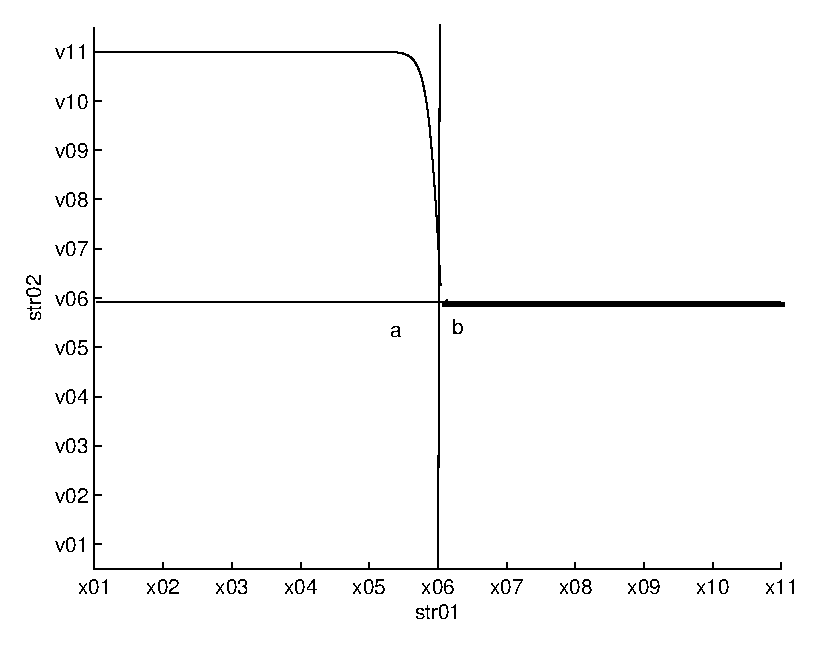
\epsfig{file=./stabilization/eps/subsidy.eps}}%
\end{psfrags}%
%
% End subsidy.tex
\end{figure}\end{document}
% See http://www.uni-kassel.de/~linne/ for recent versions of laprint.m.
%
% created by:           LaPrint version 2.03 (19.1.2000)
% created on:           13-Oct-2009 13:15:05
% options used:         / noextrapicture
% latex width:          12 cm
% factor:               0.8
% eps file name:        subsidy.eps
% eps bounding box:     15 cm x 11.25 cm
% comment:              
%
\begin{psfrags}%
\psfragscanon%
%
% text strings:
\psfrag{str03}[t][t]{x}%
\psfrag{str04}[b][b]{Subsidy factor: $-tanh(x-b)$}%
%
% xticklabels:
\psfrag{x01}[t][t]{-6}%
\psfrag{x02}[t][t]{-4}%
\psfrag{x03}[t][t]{-2}%
\psfrag{x04}[t][t]{0}%
\psfrag{x05}[t][t]{2}%
\psfrag{x06}[t][t]{4}%
\psfrag{x07}[t][t]{6}%
%
% yticklabels:
\psfrag{v01}[r][r]{-1}%
\psfrag{v02}[r][r]{-0.8}%
\psfrag{v03}[r][r]{-0.6}%
\psfrag{v04}[r][r]{-0.4}%
\psfrag{v05}[r][r]{-0.2}%
\psfrag{v06}[r][r]{0}%
\psfrag{v07}[r][r]{0.2}%
\psfrag{v08}[r][r]{0.4}%
\psfrag{v09}[r][r]{0.6}%
\psfrag{v10}[r][r]{0.8}%
\psfrag{v11}[r][r]{1}%
%
% Figure:
\resizebox{12cm}{!}{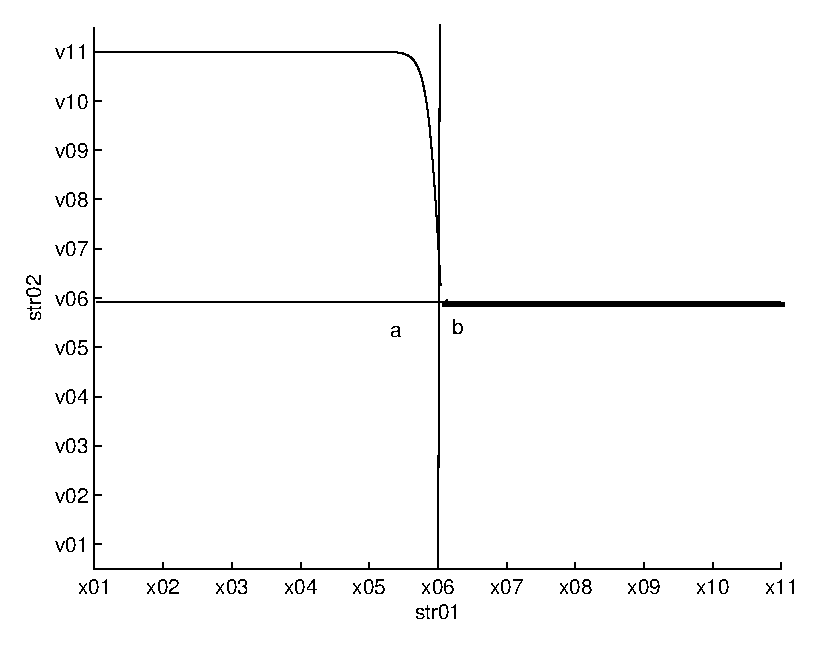
\epsfig{file=./stabilization/eps/subsidy.eps}}%
\end{psfrags}%
%
% End subsidy.tex
\end{figure}\end{document}
% See http://www.uni-kassel.de/~linne/ for recent versions of laprint.m.
%
% created by:           LaPrint version 2.03 (19.1.2000)
% created on:           05-Oct-2009 13:45:58
% options used:         / noextrapicture
% latex width:          12 cm
% factor:               0.8
% eps file name:        subsidy.eps
% eps bounding box:     15 cm x 11.25 cm
% comment:              
%
\begin{psfrags}%
\psfragscanon%
%
% text strings:
\psfrag{str01}[t][t]{x}%
\psfrag{str02}[b][b]{subsidy factor (-tanh(x-b))}%
%
% xticklabels:
\psfrag{x01}[t][t]{-25}%
\psfrag{x02}[t][t]{-20}%
\psfrag{x03}[t][t]{-15}%
\psfrag{x04}[t][t]{-10}%
\psfrag{x05}[t][t]{-5}%
\psfrag{x06}[t][t]{0}%
\psfrag{x07}[t][t]{5}%
\psfrag{x08}[t][t]{10}%
\psfrag{x09}[t][t]{15}%
\psfrag{x10}[t][t]{20}%
\psfrag{x11}[t][t]{25}%
%
% yticklabels:
\psfrag{v01}[r][r]{-1}%
\psfrag{v02}[r][r]{-0.8}%
\psfrag{v03}[r][r]{-0.6}%
\psfrag{v04}[r][r]{-0.4}%
\psfrag{v05}[r][r]{-0.2}%
\psfrag{v06}[r][r]{0}%
\psfrag{v07}[r][r]{0.2}%
\psfrag{v08}[r][r]{0.4}%
\psfrag{v09}[r][r]{0.6}%
\psfrag{v10}[r][r]{0.8}%
\psfrag{v11}[r][r]{1}%
%
% Figure:
\resizebox{12cm}{!}{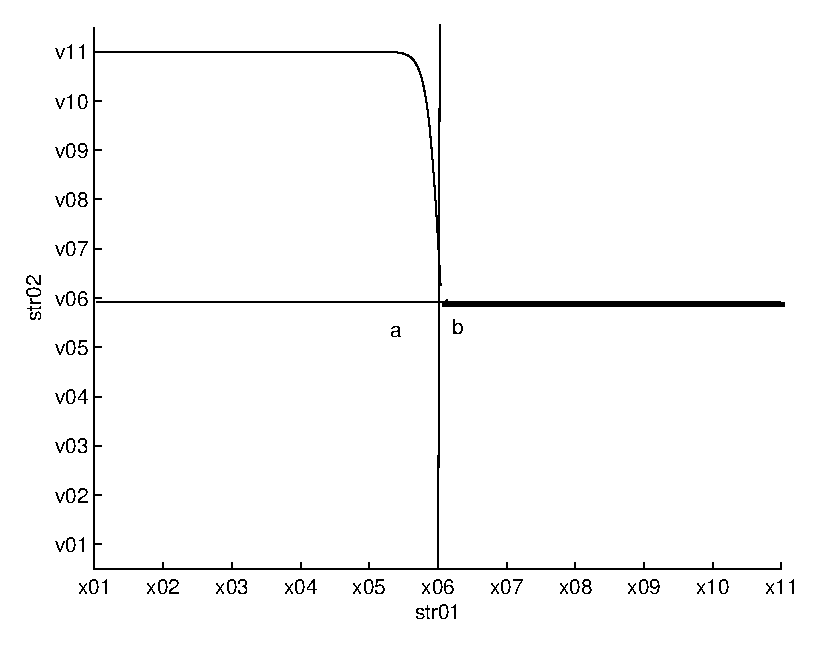
\epsfig{file=./stabilization/eps/subsidy.eps}}%
\end{psfrags}%
%
% End subsidy.tex
